\documentclass[a4paper]{book}

\usepackage[english,french]{babel}
\usepackage{amsmath}
\usepackage{amsfonts}
\usepackage{rotating}
\usepackage{multicol}
\usepackage{color}
\usepackage{verbatim}
\usepackage{hyperref}
\usepackage{float}
\usepackage{listings}
%\usepackage{cprotect}
\usepackage{fancyvrb}
\usepackage{color}
%for subfigure using ?
\usepackage{graphicx}
\usepackage{caption}
\usepackage{subcaption}
\usepackage{makeidx}

\makeindex



%\usepackage{subfigure}


\setlength{\oddsidemargin}{0.5 cm}
\setlength{\evensidemargin}{-0.5 cm}
\setlength{\textwidth}{16.0 cm}
\setlength{\textheight}{23.7 cm}
\setlength{\marginparwidth}{0.0 cm}
\setlength{\topmargin}{-1.0 cm}


%\usepackage{mathabx}
%\usepackage{amstext}
%\usepackage{amssymb}
%\usepackage{ae}


\setcounter{tocdepth}{4}
\setcounter{secnumdepth}{4}



%---------------------------------------------
\newcommand{\CPP}{\mbox{\tt C\hspace{-0.05cm}\raisebox{0.2ex}{\small ++} }}
\newcommand{\SiftPP}{\mbox{\tt Sift\hspace{-0.05cm}\raisebox{0.2ex}{\small ++} }}


\newcommand{\tran}{\ensuremath {^{t} }}
\newcommand{\trans}{\ensuremath {^{t} \!}}
\newcommand{\transs}{\ensuremath {^{t} \!\!}}
\newcommand{\transss}{\ensuremath {^{t} \!\!\!}}


\newcommand{\transL}{{\transs L}}
\newcommand{\transK}{{\transs K}}
\newcommand{\transX}{{\transs X}}
\newcommand{\transY}{{\transs Y}}

\newcommand{\transLm}{\ensuremath {\transs L^m}}
\newcommand{\transKm}{\ensuremath {\transs K^m}}
\newcommand{\KmtKm}{\ensuremath { K^m \, \transKm}}
\newcommand{\LmtLm}{\ensuremath { L^m \, \transLm}}

\newcommand{\KTH}{\ensuremath {^{th}}}
\newcommand{\EME}{\ensuremath {^{i\grave eme}}}
\newcommand{\ETer}{\ensuremath {\mathcal T}}
\newcommand{\EIm}{\ensuremath {{\mathcal I}_k}}
\newcommand{\EPx}{\ensuremath{{\mathcal E}_{px}}}

\newcommand{\FPx}{\ensuremath{{\mathcal F}_{px}}}

\newcommand{\Ok}{\ensuremath{{\mathcal O}_{k}}}

\newcommand{\Ess}{\ensuremath{{\mathcal E}}}

\newcommand{\DimPx}{\ensuremath{D_{px}}}

\newcommand{\PiI}{\ensuremath{\dot{\pi}}}
\newcommand{\PxMoy}{\ensuremath{\tilde{P_x}}}
\newcommand{\PxZone}{\ensuremath{P_x^Z}}

\newcommand{\RR}{\ensuremath{\mathbb{R}}}
\newcommand{\ZZ}{\ensuremath{\mathbb{Z}}}
\newcommand{\NN}{\ensuremath{\mathbb{N}}}
\newcommand{\Ind}{\ensuremath{\mathbb{I}^{nd}}}

\newcommand{\Ress}{\ensuremath{{\mathcal A}}}
\newcommand{\Reg}{\ensuremath{{\mathcal R}^{eg}}}
\newcommand{\Energ}{\ensuremath{{\mathcal E}}}
\newcommand{\Echant}{\ensuremath{{\mathcal E}}}
\newcommand{\PZero}{\ensuremath{{\mathcal P}^0}}
\newcommand{\SUn}{\ensuremath{{\mathcal S}^1}}

\newcommand{\DeltaI}{\ensuremath{\Delta^{\imath}}}

\newcommand{\DdSt}{\ensuremath{d^2}_{/\mathcal{S}^3}}
\newcommand{\DeuxExtre}{\ensuremath{\unrhd}}
%\newcommand{\DeuxExtre}{\ensuremath{\nabla}}
\newcommand{\RefFantome}{{\bf ?2Def?}}
\newcommand{\PourLecteurAverti}{{\Large \bf \emph{Ce paragraphe peut
facilement \^etre omis
en premi\`ere lecture.}}}
\newcommand{\COM}[1]

%  \verb|\|


\newcommand{\ELISE}
{\mbox{{\bf $\mathcal{E}$}\hspace{-0.15em}\raisebox{-0.4ex}{L}\hspace{-0.3em}\raisebox{0.3ex}{i}\raisebox{-0.4ex}{S}\raisebox{0.0ex}{e}}}

%\newcommand{\UNCLEAR}[1]{\textcolor{red}{\textbf{#1}}}
\newcommand{\UNCLEAR}{}
\newcommand{\ISITCLEAR}{}
\newcommand{\PPP}{MMVII}
\newcommand{\CdPPP}{{\tt MMVII}}
\newcommand{\MMVIDIR}{{\tt MMVII-MainFolder/}}
\newcommand{\doxy}{\emph{doxygen}}
\newcommand{\MMNONE}{NONE}

%---------------------------------------------
\begin{document}
\selectlanguage{english}

%\title{MicMac, Apero, Pastis and Other Beverages. The documentation!}
\title{Project 2007}
%\author{MPD}

\maketitle

\tableofcontents


%###########################################################################################################
%###########################################################################################################
%---------------------------------------------- PART I -----------------------------------------------------
%###########################################################################################################
%###########################################################################################################

\part{Generalities}



%   ------------------------------------------------------------------
%   ------------------------------------------------------------------
%                 Chapter set editing
%   ------------------------------------------------------------------
%   ------------------------------------------------------------------

\chapter{My first command : set editing}

%   - - - - - - - - - INTRODUCTION - - - - - - - - - - - - - - - - - -
%   - - - - - - - - - INTRODUCTION - - - - - - - - - - - - - - - - - -
%   - - - - - - - - - INTRODUCTION - - - - - - - - - - - - - - - - - -

\section{Introduction}

This chapter presents the first commands of \PPP . It uses a plan that will be almost
systematic in many other chapter :

\begin{itemize}
   \item a section relative to algorithmic and photogrammetric aspect of the chapter, generally this
         section may exist \footnote{i.e. may be of interest for the reader, hopefully}
         almost totally independantly of \PPP, but it is pre-requisite as
         there is obviously no interest to know the command and the code if the fundamentalls are
         not understood;

   \item a  user's guide section, relative to \PPP\ at user level, including the syntax of the command;

   \item one or more   programmers  section, relative to \CPP code implemanting the command, it will be a
         presentation of general organisation \footnote{as link between concept and classes},
         as the detail are to be found in \doxy pages;

\end{itemize}

This chapter will be a bit specific as the part or user's guide and programming will be much more important 
than other for a single command, as many concept common to all command will be explained here,
conversely  the algorithmic part will be very short.

%   - - - - - - - - - ALGORITHM - - - - - - - - - - - - - - - - - -
%   - - - - - - - - - ALGORITHM - - - - - - - - - - - - - - - - - -
%   - - - - - - - - - ALGORITHM - - - - - - - - - - - - - - - - - -

\section{Algorithms/Photogrammetry}

This command is useful for editing a set of files.
Almost all commands of \PPP require as parameter one or more set of 
file (i.e. the subset of images that we are considering for a given computation).
For single case, this set of file can be simply specified by a regular expression :
for example {\tt ".*JPG"} to specify all the file with a {\tt JPG} extension.

However for more complex case we may want to :

\begin{itemize}
   \item  create a set from a single pattern;
   \item  add or substract an interval, a pattern \dots
   \item  memorize the result and reuse it.
\end{itemize}


This is what does the  {\tt EditSet} command, piece by piece create a
{\tt XML} file that memorize a "complex" set of file that can be used
instead of a pattern.

%   - - - - - - - - - USER'S GUIDE 1 - - - - - - - - - - - - - - - - - -
%   - - - - - - - - - USER'S GUIDE 1- - - - - - - - - - - - - - - - - -
%   - - - - - - - - - USER'S GUIDE 1- - - - - - - - - - - - - - - - - -

\section{User's side(1)}
\index{EditSet}

    % = = = = = = = = = = = = = = = = = = = = = = =

\subsection{Basic notion }

\PPP\, is a command line programm. There is unique programm which
name is \CdPPP. Any command, {\tt OneCmd}, of \PPP\, will be called with the 
syntax {\tt  \CdPPP\,  OneCmd Args} where {\tt Args} are the arguments
of the command. To know what are the existing command there is two way :

\begin{itemize}
   \item  a basic one just enter  {\tt  \CdPPP};
   \item  a more sophisticated one , to be written,  {\tt  \CdPPP\, help}
          described in~\ref{HelpCmd};
\end{itemize}

For the basic one we get:

\begin{verbatim}
MMVII
... 
Bench => This command execute (many) self verification on MicMac-V2 behaviour
Cpp11 => This command execute some test for to check my understanding of C++11
TBS => This command execute some experiments en boost serrialization
MPDTest => This used a an entry point to all quick and dirty test by MPD ...
EditSet => This command is used to edit set of file
EditRel => This command is used to edit set of pairs of files
...
\end{verbatim}

We get the list of all command and short commentary on the service given by
the command.

    % = = = = = = = = = = = = = = = = = = = = = = =

\subsection{Getting help}

Very currently, user will know what the command does, but will not remember the exact syntax.
The {\tt help} key word can be used at any position for requiring this information,
for example :

\begin{verbatim}
MMVII EditSet help

**********************************
*   Help project 2007/MMVII      *
**********************************

  For command : EditSet 
   => This command is used to edit set of file
   => Srce code entry in :../../MMVII/src/Appli/cMMVII_CalcSet.cpp

 == Mandatory unnamed args : ==
  * string [FDP] :: Full Name of Xml in/out
  * string :: Operator in (+= *= -= = =0)
  * string [MPI0] :: Pattern or Xml for modifying

 == Optional named args : ==
  * [Name=Show] int :: Show detail of set before/after , (def) 0->none, (1) modif, (2) all
  * [Name=Out] string :: Destination, def=Input, no save for NONE
\end{verbatim}

We get three part :


\begin{itemize}
   \item  first part give the short comment, and the name of the \CPP file where
          the entry point of the command is implemented (may be of interest to programmers);

   \item  second part contains the description of mandatory args, we see that here we
          have three mandatory args;  for each args is indicated the type (here all strings),
          and  after {\tt ::}, the semantic of the parameter;
          sometime it is inserted  inside square bracket (like {\tt [FDP]}) some "predefined semantics"
          that will be described later (~\ref{Param:Pred:Sem});

   \item  third part contains the description of optional args, as for mandatory args, 
          the type and a short command is given, before this is added the name the optional
          parameter in the form {\tt [Name=TheName]};
\end{itemize}



As said before, {\tt help} can appear at any position after {\tt OneCmd}, this can be 
usefull when one has begin to edit a command, and dont want to loose it, for example
with parameter of next section, the following line is perfectly valide to obtain
help about   {\tt EditSet} :

\begin{verbatim}
MMVII EditSet File.xml = "F[0-3].txt" help
\end{verbatim}

    % = = = = = = = = = = = = = = = = = = = = = = =

\subsection{basic usage}

For example, if we go in the folder  {\tt {\MMVIDIR}MMVII-TestDir/Input/Files}, we can test :

\begin{verbatim}
MMVII EditSet File.xml = "F[0-3].txt"
\end{verbatim}

Here we have used  only the mandatory paramaters. As there is no naming for these parameters,
the order is used to make the correspondance between parameters
and value, so here :

\begin{itemize}
   \item  {\tt File.xml} correspond to first parameter described as {\tt "Full Name of Xml in/out"};
   \item  {\tt =} correspond to second paramater, described as {\tt  Operator \dots};
   \item  {\tt "F[0-3].txt"} correspond to third paramater, described as {\tt Pattern \dots};
\end{itemize}

Some comment on the effect of this parameter :
\begin{itemize}
   \item  {\tt File.xml} is the name of the {\tt XML} file  that contain the initial list of name, 
          it's pefectly acceptable that this file does not exist, in this case an empty list
          is created;

   \item  {\tt =} correspond to second paramater, is describe the operator that will be used to
          modify the file with the value $S3$ of third parameter,  its value must belong to an enumarated list with the following
          meaning
\begin{enumerate}
   \item[{\bf =}]  , $S3$ ovewrite    {\tt File.xml} ;
   \item[{\bf +=}] ,  $S3$ is added to {\tt File.xml} ;
   \item[{\bf -=}] , $S3$ is subsbracted from  {\tt File.xml}
   \item[{\bf *=}] , {\tt File.xml} is the intersection of $S3$ and its previous value;
   \item[{\bf =0}] , {\tt File.xml} is empty, whatever may be in  $S3$ ;
\end{enumerate}

   \item  {\tt "F[0-3].txt"} correspond to third paramater, described as {\tt Pattern \dots};
\end{itemize}


We can now inspect the file {\tt File.xml} which contains the name of the files
\emph{present in the folder} and matching the regular expression  {\tt "F[0-3].txt"}:

\begin{verbatim}
cat File.xml
<?xml version="1.0" encoding="ISO8859-1" standalone="yes" ?>
<MMVII_Serialization>
   <SetOfName>
      <Nb>4</Nb>
      <el>F0.txt</el>
      <el>F1.txt</el>
      <el>F2.txt</el>
      <el>F3.txt</el>
   </SetOfName>
</MMVII_Serialization>
\end{verbatim}

As always when  a regular expression is used to specify set of file,
it is understood as a filter on existing file. So if one had used {\tt "F([0-3]|[a-z]).txt"},
given the file present in  {\tt {\MMVIDIR}MMVII-TestDir/Input/Files}, we woul have
obtained exactly the same result.

\subsubsection{Exercices}
Try the following command and inspect the result , after each :

\begin{verbatim}
MMVII EditSet File.xml  = "F[0-3].txt"
MMVII EditSet File.xml += "F[7-9].txt"
MMVII EditSet File.xml -= "F8.txt"
MMVII EditSet File.xml *= "F[02468].txt"
MMVII EditSet File.xml =0 ".*"
\end{verbatim}

    % = = = = = = = = = = = = = = = = = = = = = = =

\subsection{Optional paramaters}

\subsubsection{{\tt Out} paramater}

Optional parameter are given after  the  mandary one in a list of 
string {\tt Name=Value}. For example until now we have use
the file {\tt File.xml} both as input and output, but sometime
we don't want to modify the input file, we can the use the optionnal
{\tt Out} parameter. For example if we enter :

\begin{verbatim}
MMVII EditSet File.xml = "F[0-3].txt" 
MMVII EditSet File.xml += "F[7-9].txt"  Out=File2.xml
\end{verbatim}

After first line {\tt File.xml} contains t$4$ names.
After second line, the  {\tt File.xml} is unchanged
while  {\tt File2.xml} contains $7$ names.


An interesting option, for this commans as each time
a pattern is expected, is that if the file is {\tt XML}
file, created by \PPP\, and with main tag {\tt <SetOfName>},
then name used will not be the pattern itself but the name
contained in the file, for example : 

\begin{verbatim}
MMVII EditSet File1.xml = "F[0-3].txt"  
MMVII EditSet File2.xml = "F[7-9].txt"  
MMVII EditSet File1.xml += File2.xml  Out=File3.xml
MMVII EditSet File3.xml += File2.xml  Out=File4.xml
\end{verbatim}

After this command {\tt File3.xml} contains the sum of {\tt File1.xml} and {\tt File2.xml},
here $7$ name. All the operation are set operation, in the mathematicall sense, so there is
no duplicate, dans {\tt File4} contain still $7$ names.

      %  -  -  -  -  -  -  -  -  -  -  -

\subsubsection{{\tt Show} paramater}

The {\tt Show} allow to visualize the result of the operation.

\begin{verbatim}
MMVII EditSet File.xml =0 ".*"
MMVII EditSet File.xml = "F[0-4].txt"
MMVII EditSet File.xml += "F[0-6].txt" Show=1
-+ F5.txt
-+ F6.txt
MMVII EditSet File.xml *= "F[02468].txt" Show=2
 ++ F0.txt
 ++ F2.txt
 ++ F4.txt
 ++ F6.txt
 +- F1.txt
 +- F3.txt
 +- F5.txt
\end{verbatim}

The third command use the parameter {\tt Show}, as the value is $1$,
only the modification are shown : 

\begin{itemize}
   \item {\tt -+ F5.txt} means that the file was inially absent ($-$) and is present at end ($+$)
\end{itemize}

It is also possible to show all the result, including the names that
present before and after the modification :

\begin{itemize}
   \item {\tt ++ F0.txt} : means that the file is present before and after the operation;
   \item {\tt +- F1.txt} : means that the file is present before and absent after the operation;
\end{itemize}


    % = = = = = = = = = = = = = = = = = = = = = = =

\subsection{More help}

In \PPP there exists many optional parameter. There are not shown by default in the help mode,
but it is possible to show :

\begin{itemize}
   \item  the standard common parameter by setting {\tt Help} instead of {\tt help}

   \item  all the common parameter, including the \emph{internal} common parameter
          by setting {\tt HELP} instead of {\tt help}; the internal parameter are used
          by \PPP to communicate information to sub-process  when  \PPP  calls itself;
          for example the parameter {\tt LevCall} allow \PPP to know if it was called
          by the user or by \PPP and to which level of imbrication; obviously it is generally
          a bad idea to fix yourself the internall parameter;
\end{itemize}

Here is an example with {\tt EditSet} :

\begin{verbatim}
MMVII EditSet File.xml *= "F[02468].txt" Show=2 HELP
...
  * [Name=Out] string :: Destination, def=Input, no save for NONE
  * [Name=FFI0] string [FFI0] :: File Filter Interval, Main Set   ### COMMON 
  * [Name=FFI1] string [FFI1] :: File Filter Interval, Second Set   ### COMMON 
  * [Name=NumVOut] int :: Num version for output format (1 or 2)   ### COMMON 
  * [Name=DirProj] string [DP] :: Project Directory   ### COMMON 
  * [Name=StdOut] string :: Redirection of Ouput (+File for add,NONEfor no out)   ### COMMON 
...
  * [Name=LevCall] int :: Internal : Don't Use !!   ### INTERNAL 
  * [Name=ShowAll] bool :: Internal : Don't Use !!   ### INTERNAL 
...
\end{verbatim}

As some command have many option, it possible to filter the
optionnal parameter using a regular expression , with a
syntax {\tt help=expr} (or {\tt Help} or {\tt HELP}), for
example :


\begin{verbatim}
MMVII EditSet File.xml *= "F[02468].txt" Show=2 HELP=F.*
...
 == Optional named args : ==
  * [Name=FFI0] string :: File Filter Interval, Main Set   ### COMMON 
  * [Name=FFI1] string :: File Filter Interval, Second Set   ### COMMON 
\end{verbatim}


%   - - - - - - - - - USER'S GUIDE GLOBAL PARAMETER - - - - - - - - - - - - - - - - - -
%   - - - - - - - - - USER'S GUIDE GLOBAL PARAMETER - - - - - - - - - - - - - - - - -
%   - - - - - - - - - USER'S GUIDE GLOBAL PARAMETER - - - - - - - - - - - - - - - - -

\section{User's side-2, global parameter}


    % = = = = = = = = = = = = = = = = = = = = = = =

\subsection{Fixing project directory {\tt DirProj}}

\label{Fix:Dir:Proj}

In \PPP\, the notion of  project is closely related to the folder where
are stored a given set of data, basically one can consider for universall the rule 
"one project/one folder".
\PPP\, uses the following rule to determine the directory of project  :

\begin{itemize}
   \item  many command have a parameter that fix the project folder,
          for example with {\tt EditSet} the first parameter fix the 
          project directory, they are indicated by {\tt [FDP]} (see~\ref{Param:Pred:Sem});

   \item  when there is no command to fix the folder, by default \PPP
          fix the project folder to {\tt "./"}.;

    \item it is also possible to fix this directory with the optionnal
          parameter  {\tt DirProj}.
\end{itemize}

For example, if we go in the folder   {\tt {\MMVIDIR}MMVII-TestDir/Input/}, we can test :

\begin{verbatim}
MMVII EditSet Files/FileX.xml = "F[0].txt"   
MMVII EditSet Files/FileX.xml = "F[0].txt"  Show=2  
 ++ F0.txt
MMVII EditSet FileX.xml = "F[0].txt"  Show=2  DirProj=Files/
 ++ F0.txt
\end{verbatim}

In the first two command, the project folder is computed from {\tt Files/FileX.xml}.
In the last command, it is computed from {\tt DirProj=Files/}.



    % = = = = = = = = = = = = = = = = = = = = = = =

\subsection{Filtering by interval {\tt FFI0}, {\tt FFI1}}

Intervall can be used for different  ordered type, for string the order
is the standard lexicographic order. Interval are describe on command
line usign square barcket, {\tt "["} and  {\tt "]"}, separated by a comma {\tt ","}.
Rather than a formal definition, explain by example :

\begin{itemize}
   \item one can use closed interval : {\tt [a100.jpg,a150.jpg]} filter the string $S$ such that   $ a100.jpg \leq S $ and  $ S \leq a100.jpg $ 
   \item one can use open interval  : {\tt ]a100.jpg,a150.jpg[} filter the string $S$ such that   $ a100.jpg <  S $ and  $ S < a100.jpg $ 
   \item interval can be semi open as  {\tt [a100.jpg,a150.jpg[} with obvious interpretation;
   \item interval can be semi finite :  {\tt [a100.jpg,[} filter the string  $ a100.jpg \leq S $, and no upper bound;
   \item finally one can create union of intervall by simply concatening the string: {\tt  ],a110jpg[ [a140.jpg,[}
         filter the string such that  $ S < a110.jpg $ \emph{or}  $  a140.jpg \leq S $
       
\end{itemize}

The common optional parameter {\tt FFI0} (and {\tt FFI1}) can be used to do this filtering,
for example , if we go in the folder  {\tt {\MMVIDIR}MMVII-TestDir/Input/Files}, we can test :

\begin{verbatim}
MMVII EditSet File.xml = "F.*txt" FFI0="[F1.txt,F3.txt[]F7.txt,["
...
      <el>F1.txt</el>
      <el>F2.txt</el>
      <el>F8.txt</el>
      <el>F9.txt</el>
\end{verbatim}

In this example, the parameter {\tt FFI0} has been used to filter {\tt "F.*txt"},
and gives the result described with the $4$ names. Of course, the question is "How the user can knows that the
filter  {\tt FFI0}  will apply to this parameter ?".  This here where comes the
"predefined semantics"  {\tt [MPI0]} that is shown in the help (see \ref{Param:Pred:Sem}).

    % = = = = = = = = = = = = = = = = = = = = = = =

\subsection{Redirecting message with {\tt StdOut}}

By defaut \PPP\, print several messages on the console. When user want  to
print the messages in a file {\tt File.txt}, it is possible to :

\begin{itemize}
  \item just append the messages at the end to the possibily existing file  by {\tt StdOut=File.txt};
  \item just append the messages to the possibily existing file  and still print the messages on the console
        by {\tt StdOut=+File.txt};
  \item print  the messages in this file, and reset if it exist, {\tt StdOut=0File.txt};
  \item print  the messages in this file, and reset if it exist, and still print the 
       messages on the console by {\tt StdOut=0+File.txt};
  \item print  nothing by {\tt StdOut=\MMNONE}.
\end{itemize}

This has for consequences that the name of the file of redirection 
cannot begin by {\tt +} or {\tt 0}.

\subsubsection{Exercices}
Try the following command and inspect the result , after each :

\begin{verbatim}
# File Mes.txt grows
MMVII EditSet File.xml  = "F[0-3].txt" StdOut=Mes.txt Show=2
MMVII EditSet File.xml  = "F[0-3].txt" StdOut=+Mes.txt Show=2
MMVII EditSet File.xml  = "F[0-3].txt" StdOut=Mes.txt Show=2
# File Mes.txt reiniliazed
MMVII EditSet File.xml  = "F[0-3].txt" StdOut=0Mes.txt Show=2
MMVII EditSet File.xml  = "F[0-3].txt" StdOut=0+Mes.txt Show=2
MMVII EditSet File.xml  = "F[0-3].txt" StdOut=+0Mes.txt Show=2
# No output
MMVII EditSet File.xml  = "F[0-3].txt" StdOut=NONE Show=2
\end{verbatim}

    % = = = = = = = = = = = = = = = = = = = = = = =


    % = = = = = = = = = = = = = = = = = = = = = = =

\subsection{Fixing MicMac version for export {\tt NumVOut}}

As versions $1$ and $2$ of MicMac will coexist for several (many ?) years,
it is usefull that new tools are able to import/export. For import, the solution
is easy, \PPP, recognize by analyzing the first tag which version is it (if any).
For export the rule are more complicated but quite logical, they use the common
optionnal parameter {\tt NumVOut} :

\begin{itemize}
    \item if {\tt NumVOut} is set (to $1$ or $2$) this fix the num version for export;
    \item else if there at least one file of $V2$ was imported, the export will be in $V2$;
    \item else if there at least one file of $V1$ was imported, the export will be in $V1$;
    \item else  the export will be in $V2$;
\end{itemize}

    % = = = = = = = = = = = = = = = = = = = = = = =

\subsection{Predefined semantics}

\label{Param:Pred:Sem}

      %  -  -  -  -  -  -  -  -  -  -  -

\subsubsection{Generalities}

Many parameters of many command of \PPP correspond to the same meaning/semantic,
this is  the case for "main set of images", "main orientation", \dots These predefined
semantic are indicated in square bracket after the types, for example with command
{\tt EditSet} we can see {\tt [FDP], [MPI0], [FFI0],[FFI1] [DP]} :


\begin{verbatim}
MMVII EditSet HELP
...
  * string [FDP] :: Full Name of Xml in/out
  * string [MPI0] :: Pattern or Xml for modifying
...
  * [Name=FFI0] string [FFI0] :: File Filter Interval, Main Set   ### COMMON 
  * [Name=FFI1] string [FFI1] :: File Filter Interval, Second Set   ### COMMON 
  * [Name=DirProj] string [DP] :: Project Directory   ### COMMON 
..
\end{verbatim}

We desribe after this semantic (but not for common parameter, as they have already been described).


      %  -  -  -  -  -  -  -  -  -  -  -

\subsubsection{Main pattern image {\tt [MPI]}}

Many command have a parameter which is the main set/pattern of files (generally images).
This  parameter is described by the predefined semantic {\tt [MPI0]}. If this
parameter exists, then  it is possible to use {\tt [FFI0]} to filter the set (if there
is no {\tt [MPI0]} then use of {\tt [FFI0]}  is forbidden).

Some command have several main sets, in this case one of their parameter will have
the predefined semantic {\tt [MPI1]}, which can be filtered by {\tt [FFI1]}. See
the command {\tt EditRel}.


      %  -  -  -  -  -  -  -  -  -  -  -

\subsubsection{File of Directory Project {\tt [FDP]}}

The notion of project directory was introduced in~\ref{Fix:Dir:Proj}.
Generally there is no need to specify it, as there is one "main" file parameter
that fix this directory. This parameter can be recognized by the predefined
semantic  {\tt [FDP]}, in {\tt EditSet} command, this is first parameter that
corresponds to this.




%   - - - - - - - - - USER'S GUIDE , FREQUENT ERROR - - - - - - - - - - - - - - - - - -
%   - - - - - - - - - USER'S GUIDE , FREQUENT ERROR - - - - - - - - - - - - - - - - - -
%   - - - - - - - - - USER'S GUIDE , FREQUENT ERROR - - - - - - - - - - - - - - - - - -

\section{User's side-3, most frequent error}


    % = = = = = = = = = = = = = = = = = = = = = = =

\subsection{Generality}

When a command fails, it generates an error message and generally wait for 
the user to press "return key".
The first part of the message contains the type of error, it can be :

\begin{itemize}
   \item {\tt Level=[Internal Error]} : this mean that some incoherence in \PPP was encontered,
         probably in this case user cannot do many thing but report to forum or devlopping team
         mentionning the complete message;

   \item {\tt Level=[UserEr:XXXX]} : this means that the error is probably due to a bad
        manipulation of the user, where {\tt XXX}  is the reference of the error;
\end{itemize}

For example :

\begin{verbatim}
MMVII EditSet File.xml = "F.*txt" ShowAll=tru

Level=[UserEr:BadBool]
Mes=[Bad value for boolean :[tru]]
\end{verbatim}

Let comment the message :

\begin{itemize}
   \item {\tt Mes=[Bad value for boolean :[tru]] } : this as short message, which will be generally
         sufficient to analyse the error, here the error occured because {\tt ShowAll} is of type
         boolean and {\tt tru} is not a valide string to create a boolean;

   \item {\tt Level=[UserEr:BadBool] } : this line indicate the reference of the error,
         this reference can be used , if the short message is unsufficient, as an entry in this
         documentation to get more information on the error;

\end{itemize}

    % = = = = = = = = = = = = = = = = = = = = = = =

\subsection{Error {\tt BadBool}}
\index{BadBool}

This error occurs when a parameter of boolean type is initialized with an unvalid string.
Valide string for boolean are : {\tt \{0,1,false,true\}} (case unsensitive).
Example, parameter {\tt ShowAll} being boolean :

\begin{verbatim}
MMVII EditSet File.xml = "F.*txt" ShowAll=tru
\end{verbatim}

    % = = = = = = = = = = = = = = = = = = = = = = =

\subsection{Error {\tt BadOptP}}
\index{BadOptP}

This error occurs when an optionnal parameter name do not match any the expected
paramater name. Example, typing {\tt AllShow} instead of {\tt ShowAll}.

\begin{verbatim}
MMVII EditSet File.xml = "F.*txt" AllShow=true
\end{verbatim}

    % = = = = = = = = = = = = = = = = = = = = = = =

\subsection{Error {\tt MultOptP}}
\index{MultOptP}

This error occurs when the same optional parameter was used several time. Example doubling the {\tt NumVOut} :

\begin{verbatim}
MMVII EditSet File.xml = ".*txt" NumVOut=1 NumVOut=1
\end{verbatim}

    % = = = = = = = = = = = = = = = = = = = = = = =

\subsection{Error {\tt OpenFile}}
\index{OpenFile}

This error occurs when \PPP cannot open a file, in read or write mode, several reason can exist :
hard disk full, rights on the file system, directory do not exist. Example :

\begin{verbatim}
MMVII EditSet File.xml = ".*txt"  Out=o/o.xml
\end{verbatim}
    % = = = = = = = = = = = = = = = = = = = = = = =

\subsection{Error {\tt InsufP}}
\index{InsufP}

This error occurs when the number of parameter is inferior to the number
of mandatory parameters.  Example, omiting the operator in {\tt EditSet}:

\begin{verbatim}
MMVII EditSet File.xml "F.*txt"
\end{verbatim}

    % = = = = = = = = = = = = = = = = = = = = = = =

\subsection{Error {\tt BadEnum}}
\index{BadEnum}

This error occurs when a string cannot create a specific enum.
Example, typing {\tt eq} instead of {\tt =} in {\tt EditSet}.

\begin{verbatim}
MMVII EditSet File.xm eq "F.*txt"
\end{verbatim}


    % = = = = = = = = = = = = = = = = = = = = = = =

\subsection{Error {\tt FileSetN}}
\index{FileSetN}

This error occurs when a File a file was expected to be a set of name and : 
the file exist (else it would be just an empty set) but is not a correct
xml file in V1 or V2 format. Exemple under {\tt {\MMVIDIR}MMVII-TestDir/Input/Files},
using the file {\tt BadFile.xml} :

\begin{verbatim}
MMVII EditSet BadFile.xml = .*txt
\end{verbatim}

    % = = = = = = = = = = = = = = = = = = = = = = =

\subsection{Error {\tt IntWithoutS}}
\index{IntWithoutS}

This error occurs when a file filter image ({\tt FFI0,FFI1}) were used but
the corresponding main pattern is not member of the command, for example :

\begin{verbatim}
MMVII EditSet BadFile.xml = .*txt FFI1=[,]
\end{verbatim}


%   - - - - - - - - - PROGRAMMER'S SIDE,  - - - - - - - - - - - - - - - - - -
%   - - - - - - - - - PROGRAMMER'S SIDE,  - - - - - - - - - - - - - - - - - -
%   - - - - - - - - - PROGRAMMER'S SIDE,  - - - - - - - - - - - - - - - - - -

\section{Programmer's side, adding a new command (1)}

In this chapter we will see the main roadmap to follow for
adding a new command in \PPP.


    % = = = = = = = = = = = = = = = = = = = = = = =

\subsection{Heriting from  {\tt cMMVII\_Appli}}

A first and easy principle is "One command/One class" and  "this class must
inherit from {\tt cMMVII\_Appli}.
In our case the class corresponding to {\tt EditSet} is the class {\tt cAppli\_EditSet}
defined in file :

\begin{itemize}
   \item  {\tt \MMVIDIR/src/cMMVII\_CalcSet.cpp}
\end{itemize}
As {\tt cMMVII\_Appli} is pure virtual class, the concrete class must override
$3$ methods :

\begin{itemize}
   \item {\tt int Exe();} : this method execute the action of the command;

   \item {\tt cCollecSpecArg2007 \& ArgObl(cCollecSpecArg2007 \&)} this method communicate the specification
         of mandatory parameters;

   \item {\tt cCollecSpecArg2007 \& ArgOpt(cCollecSpecArg2007 \&)} this method communicate the specification
         of optional parameters;
\end{itemize}


    % = = = = = = = = = = = = = = = = = = = = = = =

\subsection{Link between name an class}

The first thing \PPP has to do is to create the object heriting
from {\tt cMMVII\_Appli} from the command name (here create a {\tt cAppli\_EditSet}
from  {\tt EditSet}). To avoid huge compilation this creation is done
without declaration of all the class in header; the philosophy is to have
"hidden"  derived class definition in ".cpp" files  and just export an allocator.
More precisely this is done via the class {\tt cSpecMMVII\_Appli} which is
the specification of an application, it contains :

\begin{itemize}
   \item an allocator function able to create a {\tt cMMVII\_Appli} from command line
         (see type {\tt tMMVII\_AppliAllocator}), here this is the function {\tt Alloc\_EditSet};

   \item the name of the command, here {\tt EditSet};

   \item the comment of the command;

   \item three vector of specification : features (what main group the command belongs to), type
         of input, type of output;  these specification are used in the {\tt help} command to 
         look for a given command (satisfying a requets of the user such that "which command deal with oriention
         and produce ply data?");

   \item the file where the spec is created (using macro {\tt \_\_FILE\_\_}) to help recovering file from 
         command name.
\end{itemize}

Once the spec is created, it must be added to vector containing all the 
specification, this is done simply by adding a line as 
\begin{itemize}
   \item {\tt  TheRes.push\_back(\&TheSpecEditSet);} 
\end{itemize}

in file {\tt src/Appli/cSpecMMVII\_Appli.cpp}.


    % = = = = = = = = = = = = = = = = = = = = = = =

\subsection{Specifying paramaters}

%% \subsubsection{Genarilities}

The specification of parameters is done by the methods {\tt ArgObl} and {\tt ArgOpt}.
They both return a {\tt cCollecSpecArg2007} with are an agregation of {\tt cSpecOneArg2007}.
A {\tt cSpecOneArg2007} contains the specification of one parameters, it is
a virtual class that contains :

\begin{itemize}
   \item  the variable that will be initialzed, this variable which can be of different type
          as it is contained in the derived classes;

   \item  a vector of predefined semantics, a predefined semantic is create from one
          enum {\tt eTA2007} and an optional additional string;
   \item  the comment associated to the parameter;
   \item  the name of the parameter (aways empty string {\tt ""} for mandatory parameters);
\end{itemize}

Let's make a brief comment with class {\tt EditSet}, first mandatory parameters :

{\small
\begin{verbatim}
cCollecSpecArg2007 & cAppli_EditSet::ArgObl(cCollecSpecArg2007 & anArgObl)
{
   return
      anArgObl
         << Arg2007(mXmlIn,"Full Name of Xml in/out",{eTA2007::FileDirProj})
         << Arg2007(mOp,"Operator in ("+StrAllVall<eOpAff>()+")" )
         << Arg2007(mPat,"Pattern or Xml for modifying",{{eTA2007::MPatIm,"0"}});
}
\end{verbatim}
}

Let's comment :

\begin{itemize}
   \item The function {\tt Arg2007} is template and adapt to the type of the
         l-value , here all the parameter are string , but could be {\tt int} \dots or
         any type pre-instatiated in {\tt cReadOneArgCL.cpp} using macrp {\tt MACRO\_INSTANTIATE\_ARG2007};

   \item the {\tt StrAllVall<eOpAff>()} function is used to generate the string of all valid operators;

   \item the first parameter will fix the project directory, we indicate this by a having
         the semantic {\tt  \{eTA2007::FileDirProj\}}

   \item the third parameter will be the first main set of file, with indicate it by
         the semantic {\tt {eTA2007::MPatIm,"0"}};
\end{itemize}

{\small
\begin{verbatim}
cCollecSpecArg2007 & cAppli_EditSet::ArgOpt(cCollecSpecArg2007 & anArgOpt)
{
  return
    anArgOpt
       << AOpt2007(mShow,"Show","Show detail of set before/after , (def) 0->none, (1) modif, (2) all",{})
       << AOpt2007(mXmlOut,"Out","Destination, def=Input, no save for " + MMVII_NONE,{});
}
\end{verbatim}
}

Here we use the template function {\tt AOpt2007},
it is used with a {\tt bool} (parameter {\tt mShow})
and a {\tt std::string} (parameter {\tt mXmlOut}).
We see also that there is one more parameter : the name of the 
parameter that MicMac user will see (here {\tt Show} or {\tt Out}).

    % = = = = = = = = = = = = = = = = = = = = = = =

\subsection{Standard access paramaters}

Many command have paramaters that have more or less the
same meaning. It is possible to avoid code redundancy
via standard acces function and/or use of predefined semantic.

\subsubsection{Reading set of name from file with {\tt  SetNameFromString}}
\subsubsection{Main sets with {\tt MainSetk}}


%% \subsubsection{Genarilities}

% -------------------
% -------------------
% -------------------


% -------------------
% -------------------
% -------------------

\chapter{Programming organisation, style ...}

\section{Naming convention}

\section{Never use {\tt std::cout, printf \dots}}

\section{Encapsulation of boost, stl ..}
\section{Error handling}
\section{Memory check}
\section{Serialization}
\section{Shared pointer}

\section{Random number}

\PPP use some pseudo random generator. As every such generator
they must be initialized with a seed.
By default , the seed is always the same to facilitate debuging.
When user wants initialization from time this must be specified 
with a negative value of parameter {\tt  SeedRand}.



\section{Enum to string}

The enum/string  conversion is a recurent problem of \CPP which
as far as I know is still an issue. A possible solution
would be to use some code genration which from easy to read
an write text file woul generate it. But I tried to limitate
the code generation in \PPP.

In file {\tt Serial/uti\_e2string.cpp} is implemanted 
the used solution , it consist  to create data for each enum
for which we want to do the conversion {\tt Serial/uti\_e2string.cpp}.





%---------------------------------------------

\chapter{Project management command}

\section{Help command}
\index{Help}

\label{HelpCmd}


\section{Bench command}


\begin{itemize}
    \item {\tt  MMVII Bench 2 }  : standard mode  for execuring all bench at level 2

    \item {\tt MMVII Bench 2 PatBench=.*Der.* Show=0}  : execute benches matchin {\tt ".*Der.*"},
          {\tt  Show} is explicite as, by default, it is set to {\tt  true} 
          when {\tt  PatBench} is set;
   
    \item {\tt MMVII Bench 1 PatBench=XXX} : pattern specified but no match, print all benche existing


    \item {\tt MMVII Bench 2 KeyBug=Debord\_M1 }  : force the generation of  a given error

    \item {\tt MMVII Bench 1 KeyBug=XXXX }  : will print all possible value for explicit error generation


    \item {\tt MMVII Bench 1 PatBench=InspectCube }  : as InspectCube is not a bench function, but 
         only print information, exact name must be set with {\tt PatBench}

\end{itemize}






{\tt MMVII Bench 2 KeyBug=XXX }  : standard mode  for execuring all bench at level 2

{\tt MMVII Bench 1 PatBench=MemoryOperation KeyBug} : pattern specified but no match, print all benche existing




\part{Methodologies}



\chapter{The "Aime" methods for Tie Points computation}


% Conclusion, on peut sans doute limiter le nombre de point avec ScaleStab
% pour filtrage a priori => genre les 500 les plus stable

%---------------------------------------------
%---------------------------------------------
%---------------------------------------------

\section{Fast recognition}

%---------------------------------------------

\subsection{Motivation}
For each image, we have computed tie points. A tie points is made
of a vector $V \in \RR^n)$ . Typically $V$ is invariant
to the main geometric deformation .  Le  $V_1$ and $V_2$
be two tie points, we note :

\begin{itemize}
   \item  $H_{om}(V_1,V_2) $ the fact that two tie points are homologous;
\end{itemize}

Given $V_1,V_2$, there is of course no no oracle that can indicate if  $H_{om}(V_1,V_2)$,
and classically we want to compute  a fast mathematical function $\Psi $ that indicate if two vector $V_1$ and $V_2$
correspond to the same tie points .  The ideal function would be such :

\begin{itemize}
   \item  $\Psi(V_1,V_2)  \iff H_{om}(V_1,V_2)$
\end{itemize}


Of course this impossible, and we introduce the miss rate  and fall out:

\begin{itemize}
   \item   miss rate , probability of $\Psi=0$ knowing $H_{om}=1$ , we note $p_m$;
   \item   fall out , probability of $\Psi=1$ knowing $H_{om}=0$, we note $p_f$;
\end{itemize}

As we cannot have the ideal function $\Psi $ such as $p_m=0$ and $p_f=0$,
we have to compromise, and depending on the circunstances, the price of the
two error, will not be the same. Typically, in indexation step,  we are especially
interested to have a low $p_f$; converselly in recognition step we are
especially interested to have a low  $p_m$.


\subsection{Bits vector}


\section{Gaussian pyramid}

\subsection{Computing $\sigma_0$}

\label{GP:SIGMA0}

The gaussian pyramid is made from a succession of image at different scale that
result from a gaussian filter. How can we justify it :

\begin {itemize} 
   \item  image $I_k$ must be at resolution  $R_k =  R_0 s ^k$,
   \item if we assimmilat  $I_0$ to a (sum of) gaussian of std dev $\sigma_0$  , $I_k$
         must be (sum of)  gaussian  $\sigma_0 * R_k$ 
   \item so we can write $I_k = I_0 \ast G(\sigma_k)$ with $\sigma_k^2 + \sigma_0^2 = (\sigma_0  R_k)^2$;
\end {itemize} 

To compute the pyramid, we need an estimation of $\sigma_0$. Which is quite natural, if the initial
image is very blured, it a high $R_0$, and the value $R_1-R_0 = (s-1)R_0$ is also high, which require
a high value for gaussian filter.

We need a way to estimate the initial value $\sigma_0$. Also it's quite arbirtrary, the way it is
done in MMVII is :


\begin {itemize} 
   \item  assimilate $I_0$ to a gaussian of  std dev $\sigma_0$;
   \item  suppose $I_0$ is well sampled (nor blurred nor aliased);
   \item we traduce it mathematically by  :
\end {itemize} 

\begin{equation}
    \int_{-\infty}^{+\infty} I_0 |x| = \frac{1}{2}
\end{equation}

Due to symetry , we can replace by integral on $[0,+\infty]$ and supresse absolute value :

\begin{equation}
    \int_{0}^{+\infty} \frac{x}{\sigma_0 \sqrt{2\pi}} e^{-\frac{x^2}{2\sigma_0^2}}  = \frac{1}{4}
\end{equation}

We integrate :

\begin{equation}
      \lbrack  \frac{-\sigma_0}{\sqrt{2\pi}} e^{-\frac{x^2}{2\sigma_0^2}}\rbrack  _{0}^{+\infty}  = \frac{1}{4}
\end{equation}

So :

\begin{equation}
      \sigma_0 = \sqrt{\frac{\pi}{8}} \simeq 0.626
\end{equation}


%----------------------------------------
%  A conserver : equations TIPE Lolo
%-----------------------------------------
\COM{
\begin{equation}
   \delta R = \frac{1}{\sigma} \frac{L}{S} = \frac{1}{\sigma}  \frac{2 \pi a }{ e \; dz} 
\end{equation}

\begin{equation}
   \phi  = \iint \overrightarrow{B} \overrightarrow{dS} 
         = B_M \cos(\omega t) \pi a^2
\end{equation}

\begin{equation}
   e = -\frac{d\phi}{dt}= B_M \omega  \sin(\omega t)  \pi a^2
\end{equation}


\begin{equation}
   d P_J = \frac{e^2}{\delta R}  
         = \frac{ (B_M \omega \pi a^2  \sin(\omega t))^2 \sigma_e dz }{2 \pi a}
\end{equation}


\begin{equation}
   <d P_J> = \frac{B_M^2 \; \omega ^2 \; \pi \; a^3 \; e \; \sigma \; dz}{4}
\end{equation}

\begin{equation}
  <P_J> =  \int_{z=0}^H <d P_J> = \frac{B_M^2 \; \omega ^2  \; \pi \;  a^3  \; e  \; \sigma  \; H}{4}
\end{equation}

\begin{equation}
  dU = \delta ^2 Q_{creee} +  \delta ^2 Q_{recue de l'air}
\end{equation}

\begin{equation}
  C dT = <P_J> dt - g 2\pi aH(T-T_a)
\end{equation}

\begin{equation}
  C = \mu c 2 \pi a e H
\end{equation}


\begin{equation}
  \mu c 2 \pi a e H \frac{dT}{dt} = \frac{B_M \omega^2 \pi a^3 e \sigma H}{4} - g 2 \pi a H (T-T_a)
\end{equation}


\begin{equation}
  \tau  \frac{dT}{dt} + T = T_{\infty}
\end{equation}


\begin{equation}
  \tau  = \frac{\mu  c e}{g}
\end{equation}

\begin{equation}
  T_{\infty} - T_a = \frac{(B_M \omega a)^2 e \sigma}{8g}
\end{equation}
}


%---------------------------------------------
%---------------------------------------------
%---------------------------------------------

\section{Matching by relaxation}

\subsection{Notations}

We have two images $I$ and $J$, and two set of characteristic points
in $I$ and $J$ :

\begin{itemize}
   \item $A_i \in I$ for $i \in [1 \cdots M]$;
   \item $B_j \in J$ for $j \in [1 \cdots N]$;
\end{itemize}

We will note $D_{Im}$ the size of the images, typically the length of the diagonal. It will be useful
when we need to set some geometric thresholds.

For each characteristic point, we have both a vector descriptor and a position in the image.
We note :

\begin{itemize}
   \item $A^v_i , B^v_i$  the vector descriptor,  
         $A^v_i, B^v_j \in \mathbb{R}^K $  were the dimension $K$
         is typically some hundreds; however here we are only interested by the fact  there exist 
         some distance $D^v$ between
         vector such that the lower the distance, the more likely is that points are homologous;
         we note $D^v(A^v_i , B^v_i) = D^v(A_i , B_i) $
   \item  $A^p_i , B^p_i$  the position ("pixels")   in images of $A$ and $B$ , 
         $A^p_i , B^p_i \in \mathbb{R}^2$
\end{itemize}


We suppose that we can convert the distance $D^v$ in the likelihood $L$ expressing  that $A$ and $B$
are homologous. For example we  use a threshold $\sigma_v$ and set :

\begin{equation}
    L(A_i,B_j) =  e^{-\frac{D^v(A_i,B_i)}{\sigma_v}} \label{EQ:LikL}
\end{equation}

The transformation from  $D^v$ to $L$  , or even the computation of $\sigma_v$
admitting of formula like \ref{EQ:LikL}, may be an issue. By the way we will admit from
now that we have the function $ L$ , probably a way to rationalize this fact
would be to "learn" it from statistic of "real" homologous points.


\subsection{Formulation}

We want to compute a matching between $A_i$ and $B_j$ that use both the "radiometric context" informations 
and the "spatial consistency" information :

\begin{itemize}
   \item radiometric context : $A_i , B_j$  are matched if, as much as possible, $L(A_i,B_j)$ is high;
   \item spatial consistency : if $A_i$ and $B_j$ are matched, then for each $A'_i$ and $B'_j$ such that ,
         $A'^p_i$ is close to $A^p_i$ and $B'^p_i$ is close to $B^p_i$ , then the likelihood
         to match $A'_i$ and $B'_j$ is higher (i.e. neighbors of my homologous are homologous of
         my neighbors);
\end{itemize}

The principle of relaxation is to compute a non-unique weighted matching and to use
the two pieces of information to iteratively re-compute new value of the weighting. Generally, at
the beginning, the "brute" information (=radiometric context) has a higher importance, and as we go
further we give more importance to relational information (=spatial consistency).

To formalize the problem we consider that we want to compute simultaneously two functions :


\begin{itemize}
   \item a discrete matching function $\psi$  such that $\psi (A_i)$ is the homologous
         of $A_i$, with possibly $\psi (A_i) = 0$  when no match is found for $A_i$,
         and we set  $L(A_i,0) = L_0$ where $L_0$ is a constant;
   \item a geometric \emph{smooth} function $\phi$ .
\end{itemize}

And the criterion on $\psi$ and $\phi$ are to  maximize global
likelihood $\mathcal L(\psi)$ (\ref{Crit:Psi})  while minimizing the
spatial incoherence $ \mathcal S(\psi,\phi)$  (\ref{Crit:PhiPsi}).


\begin{equation}
    \mathcal L(\psi) = \sum  L(A_i,\psi(A_i)) \label{Crit:Psi}
\end{equation}


\begin{equation}
    \mathcal S(\psi,\phi) = \sum  | \psi(A_i)^p - \phi(A^p_i) | \label{Crit:PhiPsi}
\end{equation}

Of course, there must be some strong regularity constraint on $\phi$ so that the
equation ~\ref{Crit:PhiPsi} is not trivial. Generally it belongs to a parametric
space of low dimension (such as similitude, homography ...).


\subsection{Simultaneous $\psi$ and $\phi$ ?}

In most general case, it is quite complicated to compute simultaneously $\psi$
and $\phi$.

\subsubsection{Classical approach}
In the most current case in photogrammetry, a first estimation $\psi_0$ is computed with a simple
strategy as :

\begin{equation}
    \psi_0(A_i) =  \underset{B_j \in J}{\operatorname{argmax}}  L(A_i,B_j) \label{ArgMax:Psi}
\end{equation}

And then $\phi$
is computed to remove false match detected as "outliers" of tested $\phi$. 
There is many tricks to have better result (like symmetric matching), but basically
this is the idea.

A particular and very common case of this simultaneous computation is the case
where $\phi$ represents epipolar geometry and is computed by Ransac. By the way in this
case, the  use of Ransac supposes that we know $\psi$ and that it contains a reasonable
proportion of false matches (typically no more than $50\%$). This case is quite common
for example with images acquired the same time (no diachronism) and tie-points resulting
from SIFT.

\subsubsection{Approach by computing $\phi$ first}

In the problem we want to tackle here, the proportion of false match we would get with
equations like~\ref{ArgMax:Psi} is much too high . So we suppose that we can first
have an \emph{approximate} value $\phi_0$ of $\phi$. We will discuss just after how we can
estimate $\phi_0$.

We have to specify that what we mean by $\phi_0$ is an approximation of $\phi$.
To understand equation~\ref{Phi0:ApproxG}  and~\label{Phi0:Appro} we must
imagine a possible scenario for $\phi$ and $\phi_0$. Typicaly $\phi$, the real
correspondence, will the combination of epipolar geometry and $3D$ scene, so according
to the scene, the $\phi$ can be  continuous or only piece-wise continuous. For $\phi_0$,
in our context it will be a function with few parameters, typically a similitude
plane computed from few points (at least $2$). 

We then formalize "$\phi_0$ approximating  $\phi$" by (see also Fig.~\ref{fig:spatial-consist}) :


\begin{equation}
     | \phi_0(A)  - \phi(A) |  < D_A  \label{Phi0:Appro}
\end{equation}

\begin{equation}
     | (\phi_0(A) - \phi_0(A')) -(\phi(A) - \phi(A')) |  < D_g +  \alpha |A-A'|  \label{Phi0:ApproxG}
\end{equation}

By extension, using equation \ref{Crit:PhiPsi} and criterion $\mathcal S$ we want to minimize,
we will set :

\begin{equation}
     | \phi_0(A)  - \psi(A) |  < D_A  \label{PsiPhi0:Appro}
\end{equation}

\begin{equation}
     | (\phi_0(A) - \phi_0(A')) -(\psi(A) - \psi(A')) |  < D_g +  \alpha |A-A'|  \label{PsiPhi0:ApproxG}
\end{equation}

\begin{figure}
\centering
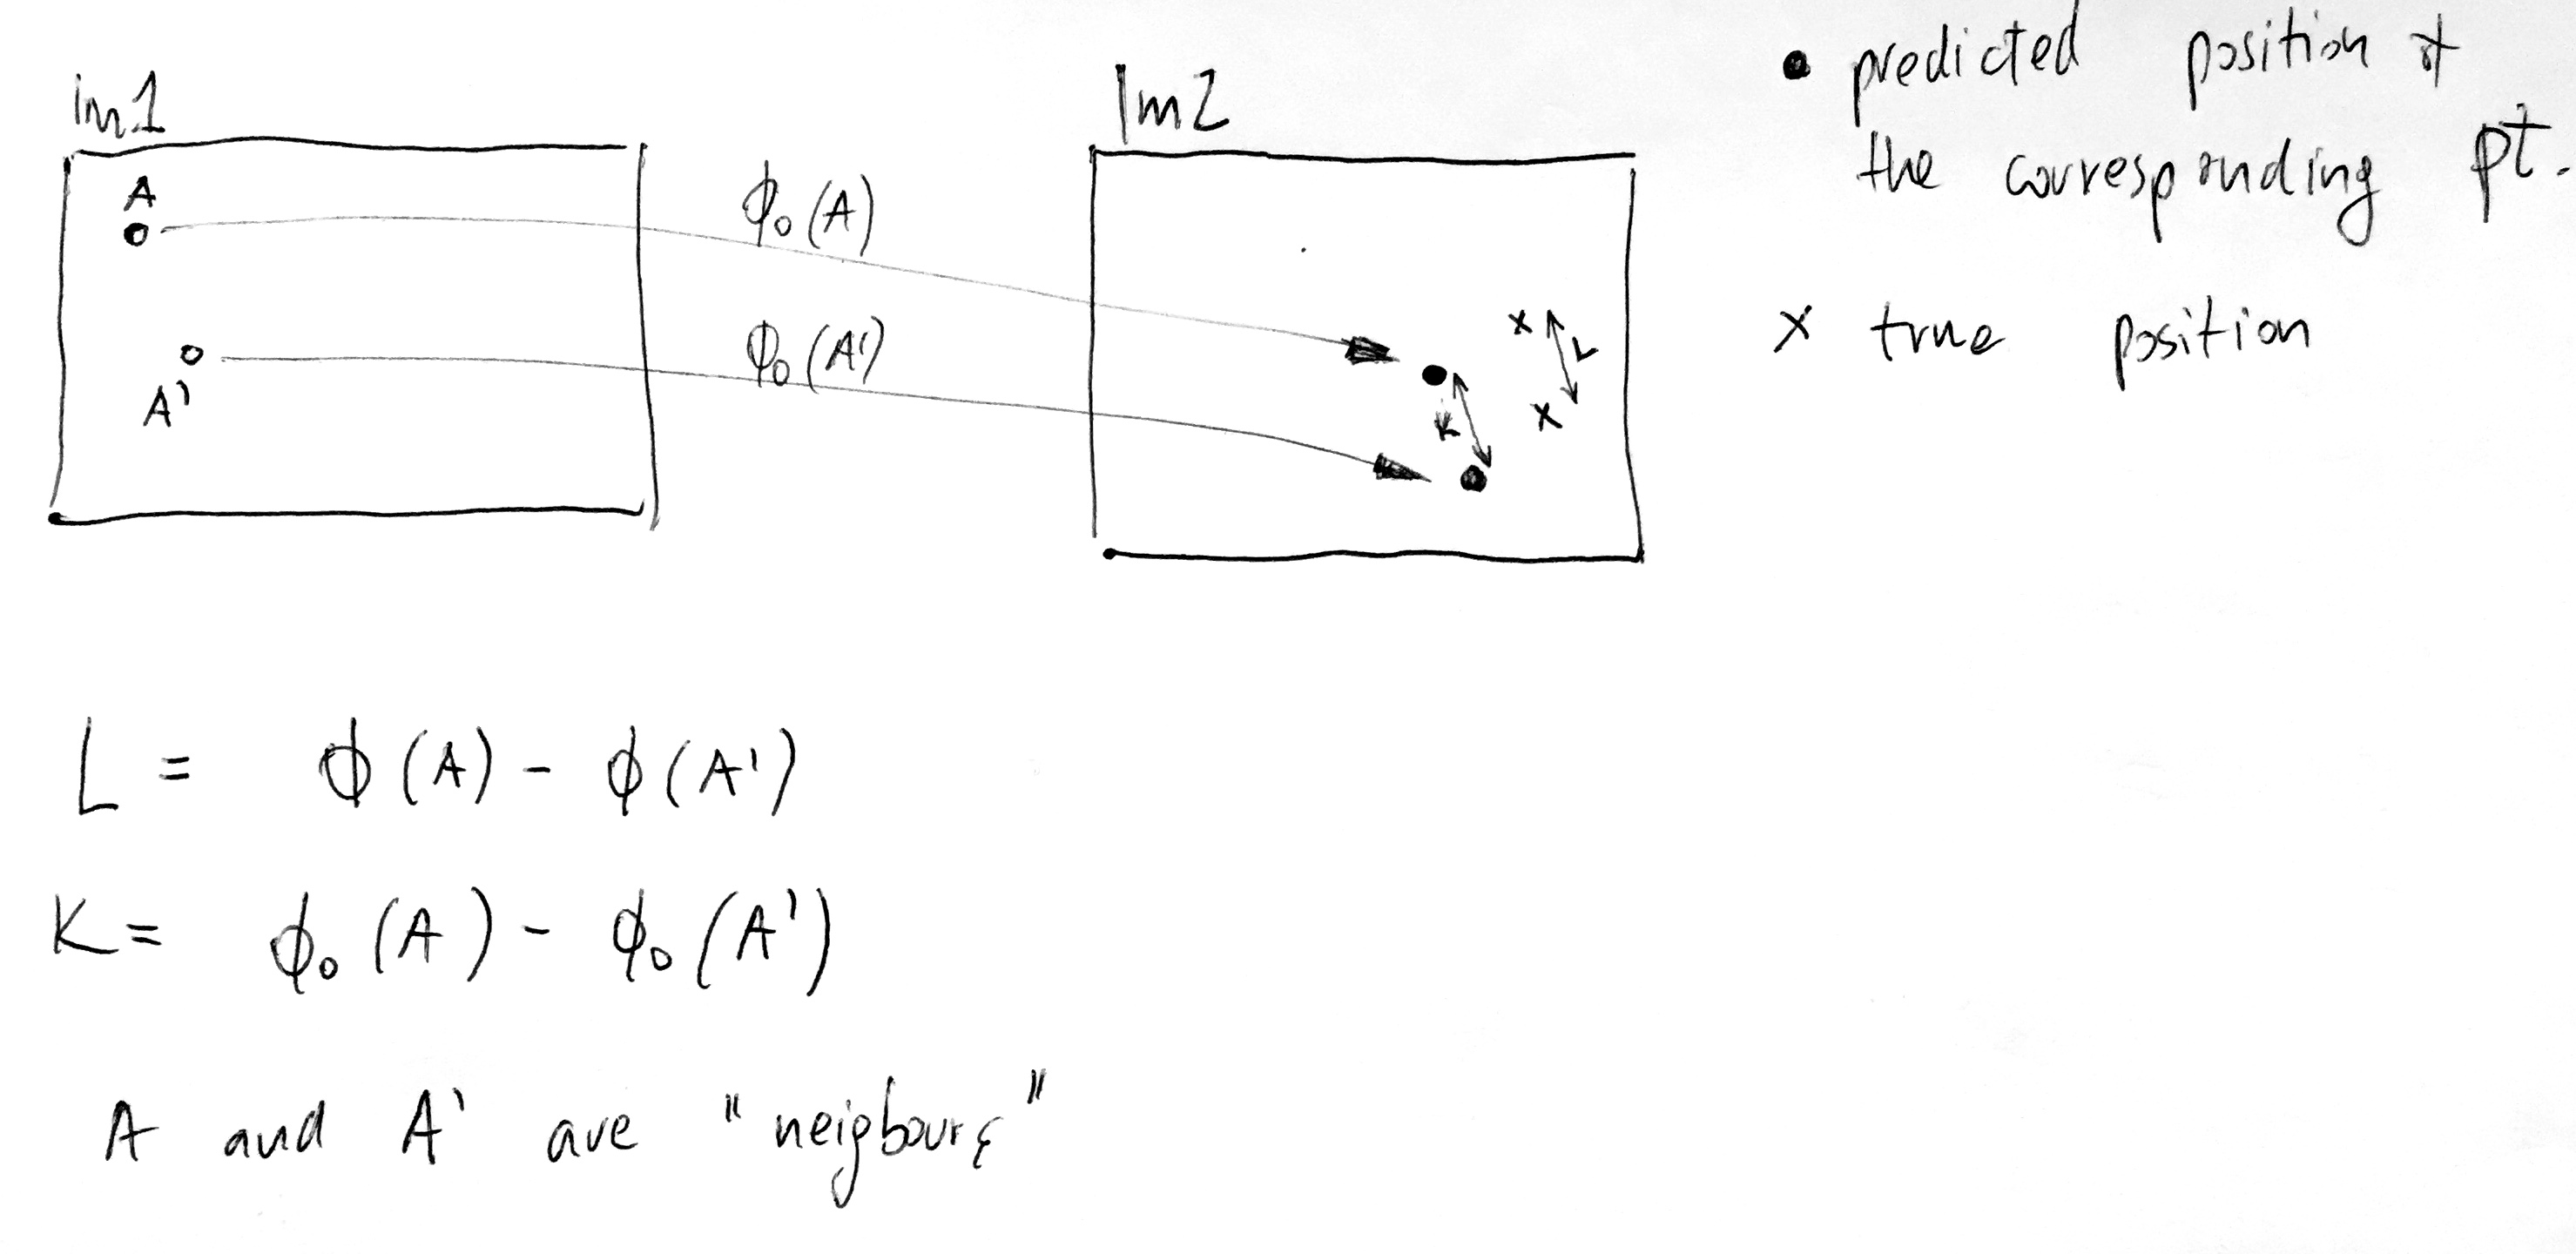
\includegraphics[width=12cm]{Methods/spatial_consist.JPG}\caption{Illustration of equation~\ref{Phi0:ApproxG}.}\label{fig:spatial-consist}
\end{figure}

Let comment these equations  :

\begin{itemize}
   \item in equations~\ref{Phi0:Appro},~\ref{PsiPhi0:Appro},~\ref{PsiPhi0Im:Appro} the value 
         $D_A$ can be relatively high as $\phi0$
         is extracted with few points and the model (similitude) is a rough approximation
         of the "real" model; it seems natural to have $D_A$ proportional to  $D_{Im}$
        (see~\ref{PsiPhi0Im:Appro});

   \item equation~\ref{Phi0:ApproxG},~\ref{PsiPhi0:ApproxG} model the fact that once 
         we "know" that  $ \psi(A)=B$ then $\phi_0$ is a relatively accurate approximation
         of $\psi$ around $A$;  when  $\phi$  is continuous, we don't need $D_g$, however
         when the $3D$ scene is discontinuous, it create discontinuities ; 
         it seems also natural to have $D_g$ proportional to  $D_{Im}$, and obviously
         $D_g$ significantly smaller than $D_A$ (see~\ref{Phi0Im:ApproxG} )
\end{itemize}

So we can write :


\begin{equation}
     | \phi_0(A)  - \psi(A) |  < \beta_A D_{Im}  \label{PsiPhi0Im:Appro}
\end{equation}

\begin{equation}
     | (\phi_0(A) - \phi_0(A')) -(\psi(A) - \psi(A')) |  < \beta_g D_{Im} +  \alpha |A-A'|  \label{Phi0Im:ApproxG}
\end{equation}

Of course, practically, an important question is the values of thresholds $\beta_A, \beta_g, \alpha $.
As a rule of thumb, values of these parameter can be fixed in the following interval :

\begin{itemize}
   \item  $\beta_A \in [0.05,0.2]$, less than $0.05$ would be very optimistic , and by the way this low
          value is probably already sufficient for basic approach like in~\ref{Basic:ArgMax};
          more than $0.2$ would be very pessimistic and by the way difficult to use;

   \item  similarly $\beta_g \in [0.01,0.05]$ and $\alpha \in [0.05,0.3]$
\end{itemize}


And in a first try I woud use $\beta_A=0.1 \;  \beta_g=0.025 \; \alpha=0.15$.


\subsection{Estimation of $\phi_0$}

Obviously, if we cannot estimate $\phi_0$, the previous stuff is useless.
Basically, we can imagine $3$ way to estimate $\phi_0$ :

\begin{itemize}
   \item  the most trivial way is to have an "external" estimation, this can come from
          meta data ("tableau d'assemblage") or from operator measurements (operator select
          manualy two real homologous point and it is sufficient to estimate a similitude);

   \item  another easy way is to use tradional Ransac on a solution like ~\ref{ArgMax:Psi}; 
          with D2Net executed at full resolution, it will probably not work as the proportion
          of false match can be very high; however it is possible to run D2Net at a very low
          resolution, where~\ref{ArgMax:Psi} works not so bad, the accuracy is not so good, but
          it is probably not a problem;

   \item  a third, more sophisticated way, consist to use a non-unique matching at high
          or medium resolution; it is described bellow .
\end{itemize}

Non-unique matching :
\begin{itemize}
   \item  for each point in one image select a number $p$ of its potential matches in the other images, in other words for each point in  $A_i$, select 
            $\Psi (A_i) $ which contains the  $B_j$ corresponding to the $p$
          best scores of $L(A_i,B_j)$; to compute $\Psi$ it is also possible to compute more globally the
          $p * M$ best pairs of all matches $(A_i,B_j)$ where $M$ is a predefined value; here, however, there might be a case where certain points are not assigned a match; to assure that all points have matches a mix of
          both approaches can be adopted (computing a global set of pairs, and also assure to have a minimal
          number of matches per point);

   \item generate solutions, by random selection, if we decide to use similitude,
         it is sufficient to use $2$ pairs of $(A_i,B_j)$  ;  it is also possible to make a biased
         random selection that favors the set of pair having higher likelihood
         (a way to do that is, for each iteration, to generate a few random pairs, 
          and finally select the the pair corresponding to the best likelihood);

   \item for each $2$ pairs, we compute a similitude $S$  and estimate it cost $C(S)$
         by formula below;

   \item after many iteration, select finaly the $S$ minizing $C(S)$.
         by formula above;

\end{itemize}

\begin{equation}
     C(S) = \sum_i (\underset{B_j \in \Psi(A_i)}{\operatorname{Min}}  c(A_i,B_j,S))
\end{equation}

For $c(A_i,B_j,S)$, different formula can be tested, a basic formula proportional to distances, 
one using a threshold to limit the influence of outliers  : 

\begin{equation}
      c(A_i,B_j,S) = Min(|S(A_i)-B_j|,D_A)
\end{equation}

Or a smoother version :

\begin{equation}
      c(A_i,B_j,S) = \frac{|S(A_i)-B_j|}{|S(A_i)-B_j|+D_A)}
\end{equation}

It is also possible to use the likelihood $L(A_i,B_j)$ and merge it with the geometric term , 
however it is always complicated to mix valures of different kind.


\subsection{Basic usage of $\phi_0$}

The easiest way to use $\phi_0$ is to re-use the basic strategy of 
equation~\ref{ArgMax:Psi} but filtering the result with  equation~\ref{Phi0:Appro}  :


\begin{equation}
   \psi_1(A_i) =  \underset{B_j \in \mathcal D(\phi_0(A_i),D_A)}{\operatorname{argmax}}  L(A_i,B_j) 
\end{equation}

Where  $\mathcal D(\phi_0(A_i),D_A)$ is  the disc of center $\phi_0(A_i)$ and radius $D_A$.

\label{Basic:ArgMax}

\subsection{Relaxation}








\chapter{Several stuff unfinished}


%---------------------------------------------
%---------------------------------------------
%---------------------------------------------

%\section{Co-variance propagation}





\COM
{
\chapter{The Fits method}

For now "bloc-note",

% Conclusion, on peut sans doute limiter le nombre de point avec ScaleStab
% pour filtrage a priori => genre les 500 les plus stable
}





%---------------------------------------------
%--------------- PART II ----------------------
%---------------------------------------------

\part{Reference documentation}



%---------------------------------------------
%--------------- PART I ----------------------
%---------------------------------------------

\part{Annexes}

\appendix

\chapter{Bibliography}


\begin{thebibliography}{AAA}
   \bibitem[Tomasi Kanabe 98]{TomKan}   S. Roy, I.J. Cox , 1998, "Shape and Motion from Image 
            Streams under Orthography: a Factorization Method", International Journal of Computer Vision, 
            9:2, 137-154 (1992)


   \bibitem[Cox-Roy 98]{CoxRoy}   S. Roy, I.J. Cox , 1998, "A Maximum-Flow
            formulation of the N-camera Stereo Correspondence
      Problem", \emph{Proc. IEEE Internation Conference on
      Computer Vision}, pp 492--499, Bombay.

   \bibitem[Fraser C. 97]{Fraser}  C. Fraser, 1997, "Digital camera self-calibration",
   \emph{ISPRS Journal of Photogrammetry and Remote Sensing}, vol. 52, issue 4, pp. 149-159,
   \bibitem[Penard L. 2006 ]{Penard}   L. Pénard, N. Paparoditis, M. Pierrot-Deseilligny.
           "Reconstruction 3D automatique de façades de bâtiments en multi-vues.",
            RFIA (Reconnaissance des Formes et Intelligence Artificielle),
            Tours, France, January 2006.
\end{thebibliography}


\printindex



\end{document}




